\section{レンズの歪曲収差とは何か}
収差を大別すると、単色収差と色収差に分けられる。歪曲収差は単色収差のひとつである。
単色収差には記述方法の異なる光線収差と波面収差の分類があるが、物理的実体は同じである。また、光線収差を求めるために、屈折面においてスネルの法則を用いて光線を追跡するとき、3次近似していくなかで、光線収差には5つの分類が出来上がる。これはザイデルの5収差と呼ばれ、歪曲収差はそのひとつとされている。
ザイデルの5収差は以下のような式で表される。このとき、物点を通るようにyz-面を選び、極座標を用いる。
\begin{eqnarray}
	\label{seidelx}
	\Delta x' & = & A r^3 \sin \theta + B r^2 y \sin 2\theta + D r y^2 \sin \theta \\
	\label{seidely}
	\Delta y' & = & A r^3 \cos \theta + B r^2 y (2+cos2\theta) + (2C+D)r y^2 \cos \theta + E y^3
\end{eqnarray}
ここで、A,B,C,D,Eは球面収差、コマ収差、非点収差、像面収差、歪曲収差を表す収差係数である。yは像高、r,\begin{math} \theta \end{math} は主平面上の極座標系で表される射出瞳の半径と長さを表す。
ここで、入射高が0のとき、つまり、r=0のときを考える。したがって、
\begin{eqnarray}
	\Delta x' & = & 0\\
	\Delta y' & = & E y^3
\end{eqnarray}
以上の式から、光軸からの像高のみに依存した項のみが残っていることがわかる。この項により表される収差を歪曲収差または、ディストーションと呼ぶ。
歪曲収差は光軸に垂直な平面上にある物体は、光軸に垂直な平面上に結像するため、像は鮮明となる。しかし、光軸から離れた部分ほど形状が歪む性質が観測できる。歪む形には糸巻き型(\begin{math}E>0\end{math})や樽型(\begin{math}E<0\end{math})が挙げられる。
歪曲収差は像点のずれが像高の3乗に比例するため、像の大きさによって横倍率が異なることにより生じる。つまり、入射光線の画角または像高により、結像倍率が異なってしまう。

\begin{figure}[h]
	\centering
	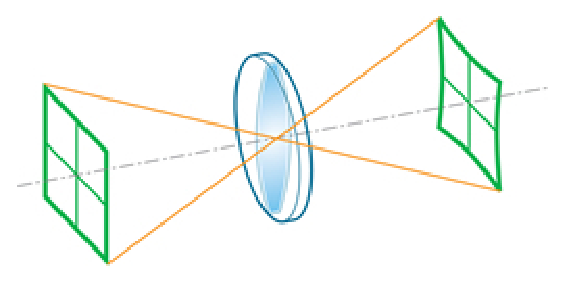
\includegraphics[height=30mm]{image/dist.png.eps}
	\caption{歪曲収差\ \cite{cite1}}
	\label{caption1}
\end{figure}

\begin{figure}[h]
    
    \centering
    \subfloat[糸巻き型]{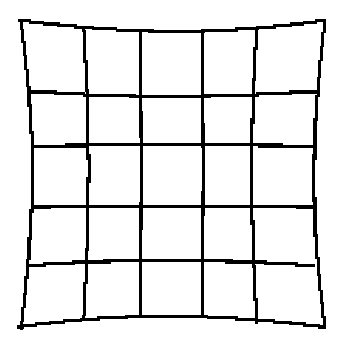
\includegraphics[height=30mm]{image/ito.png.eps} \label{shape1}}\ \ \ 
    \subfloat[樽型]{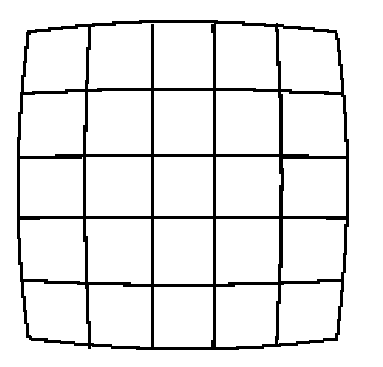
\includegraphics[height=30mm]{image/taru.png.eps} \label{shape2}}
    
    \caption{歪曲収差による観測できる形}
    \label{shape}
\end{figure}